\chapter{Raw Data}


Data Flow \newline
Block Diagram
- With different stages.
- With Data Inputs and Data Outputs of each stage. (Zoom in Diagram)

\begin{figure*}
	\begin{center}
		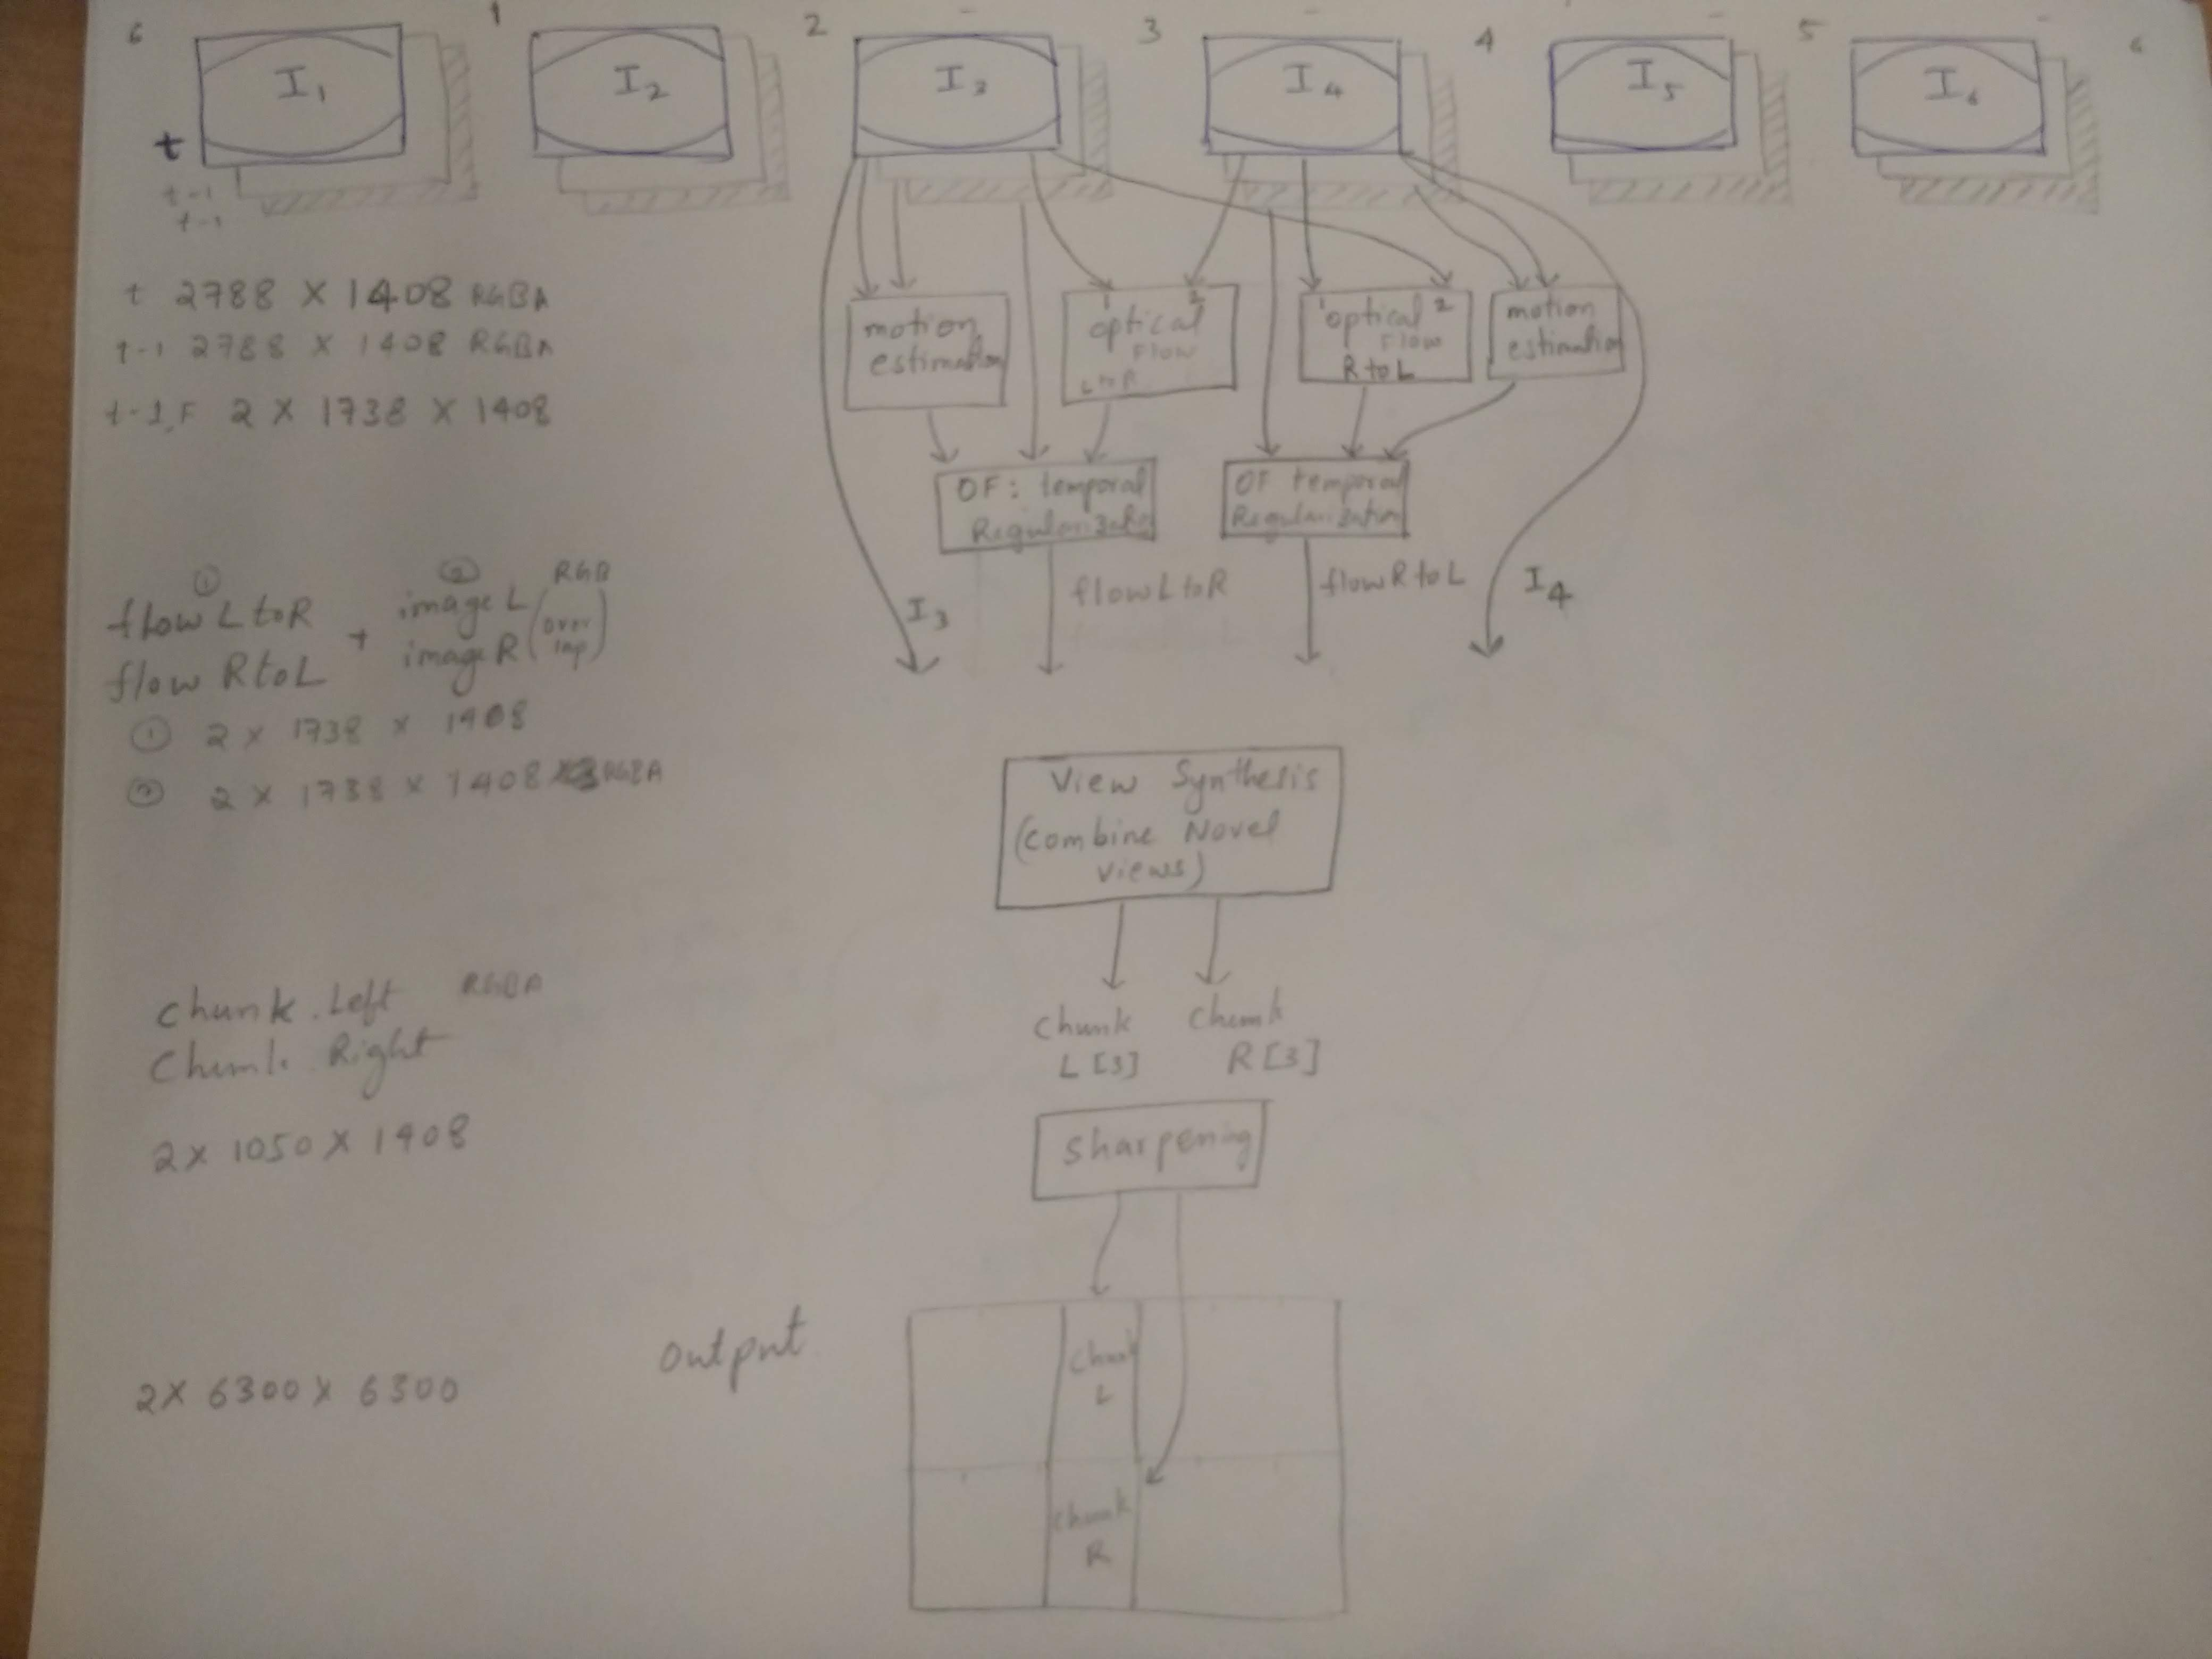
\includegraphics[width=1\textwidth]{/media/gunman/Data/thesis/ThesisLatex/data/images/ODS_Input_Output.jpg}
		\caption{X-axis shows the pyramid level and Y-axis the runtime tile search and propagate.}
		\label{ODS_Input_Output}
	\end{center}
	\vspace{-0.3in}
\end{figure*} 

The fisheye camera images.

\begin{figure*}
	\begin{center}
		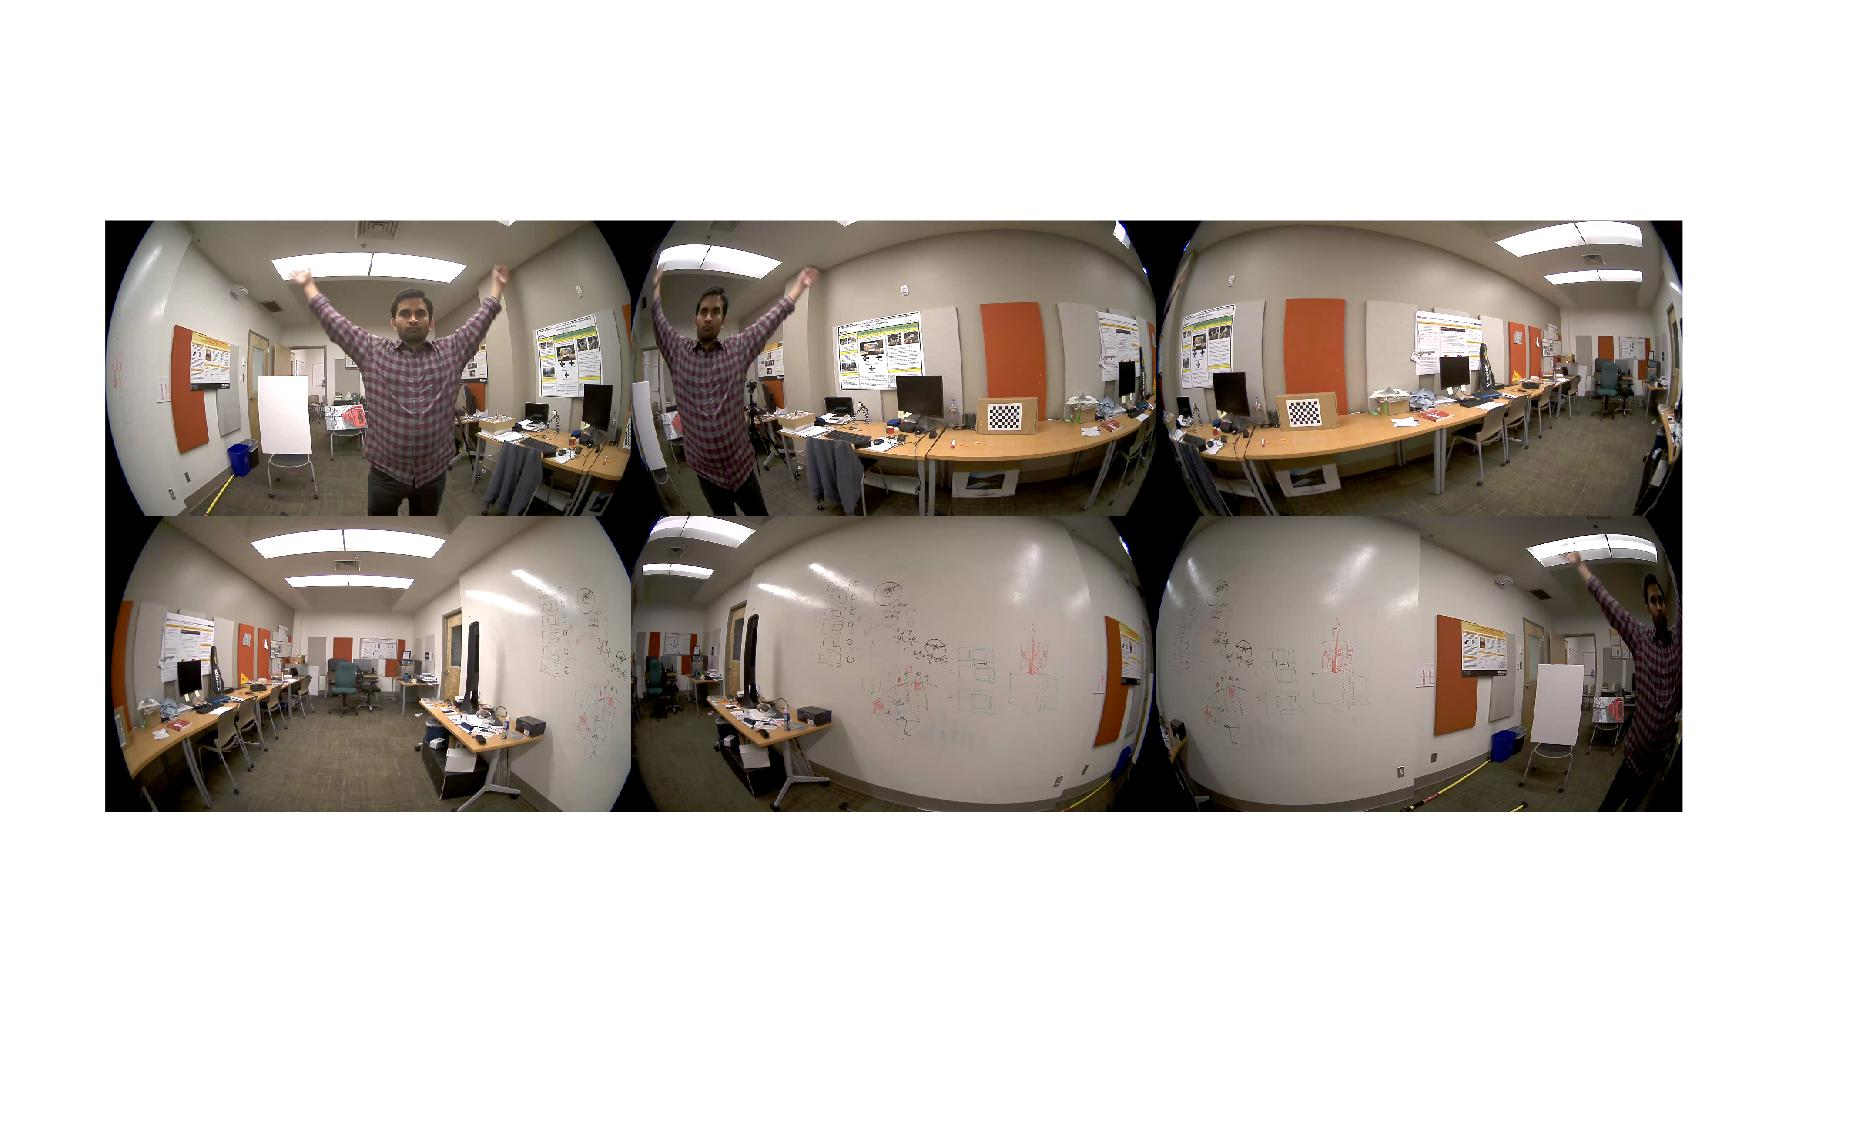
\includegraphics[width=1.1\textwidth]{/media/gunman/Data/thesis/ThesisLatex/data/images/fisheye_all6.jpg}
		\caption{Six fisheye images as captured by the IMX274 using Jetson TX2 board.}
		\label{ODS_Input_Output}
	\end{center}
	\vspace{-0.3in}
\end{figure*} 

The Equirectangular projection.

\begin{figure*}
	\begin{center}
		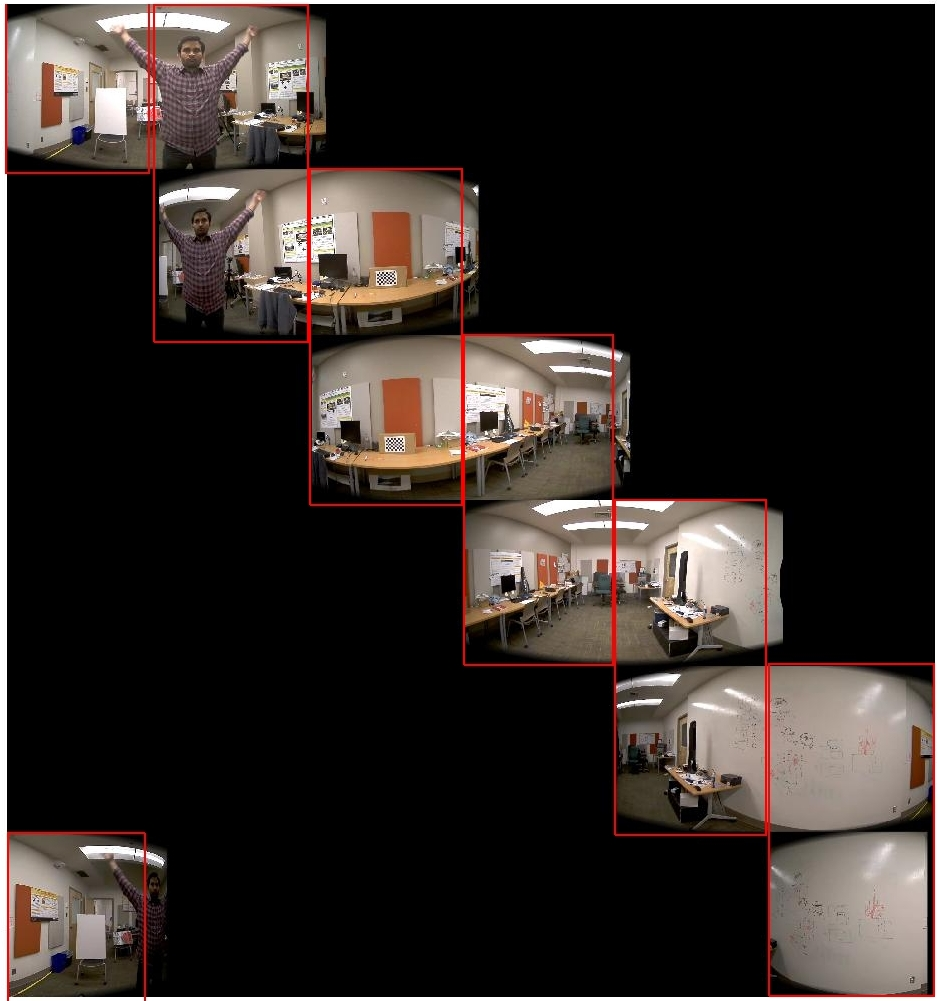
\includegraphics[width=1.5\textwidth]{/media/gunman/Data/thesis/ThesisLatex/data/images/EqRect_offset_fov_viz_loop v3.jpg}
%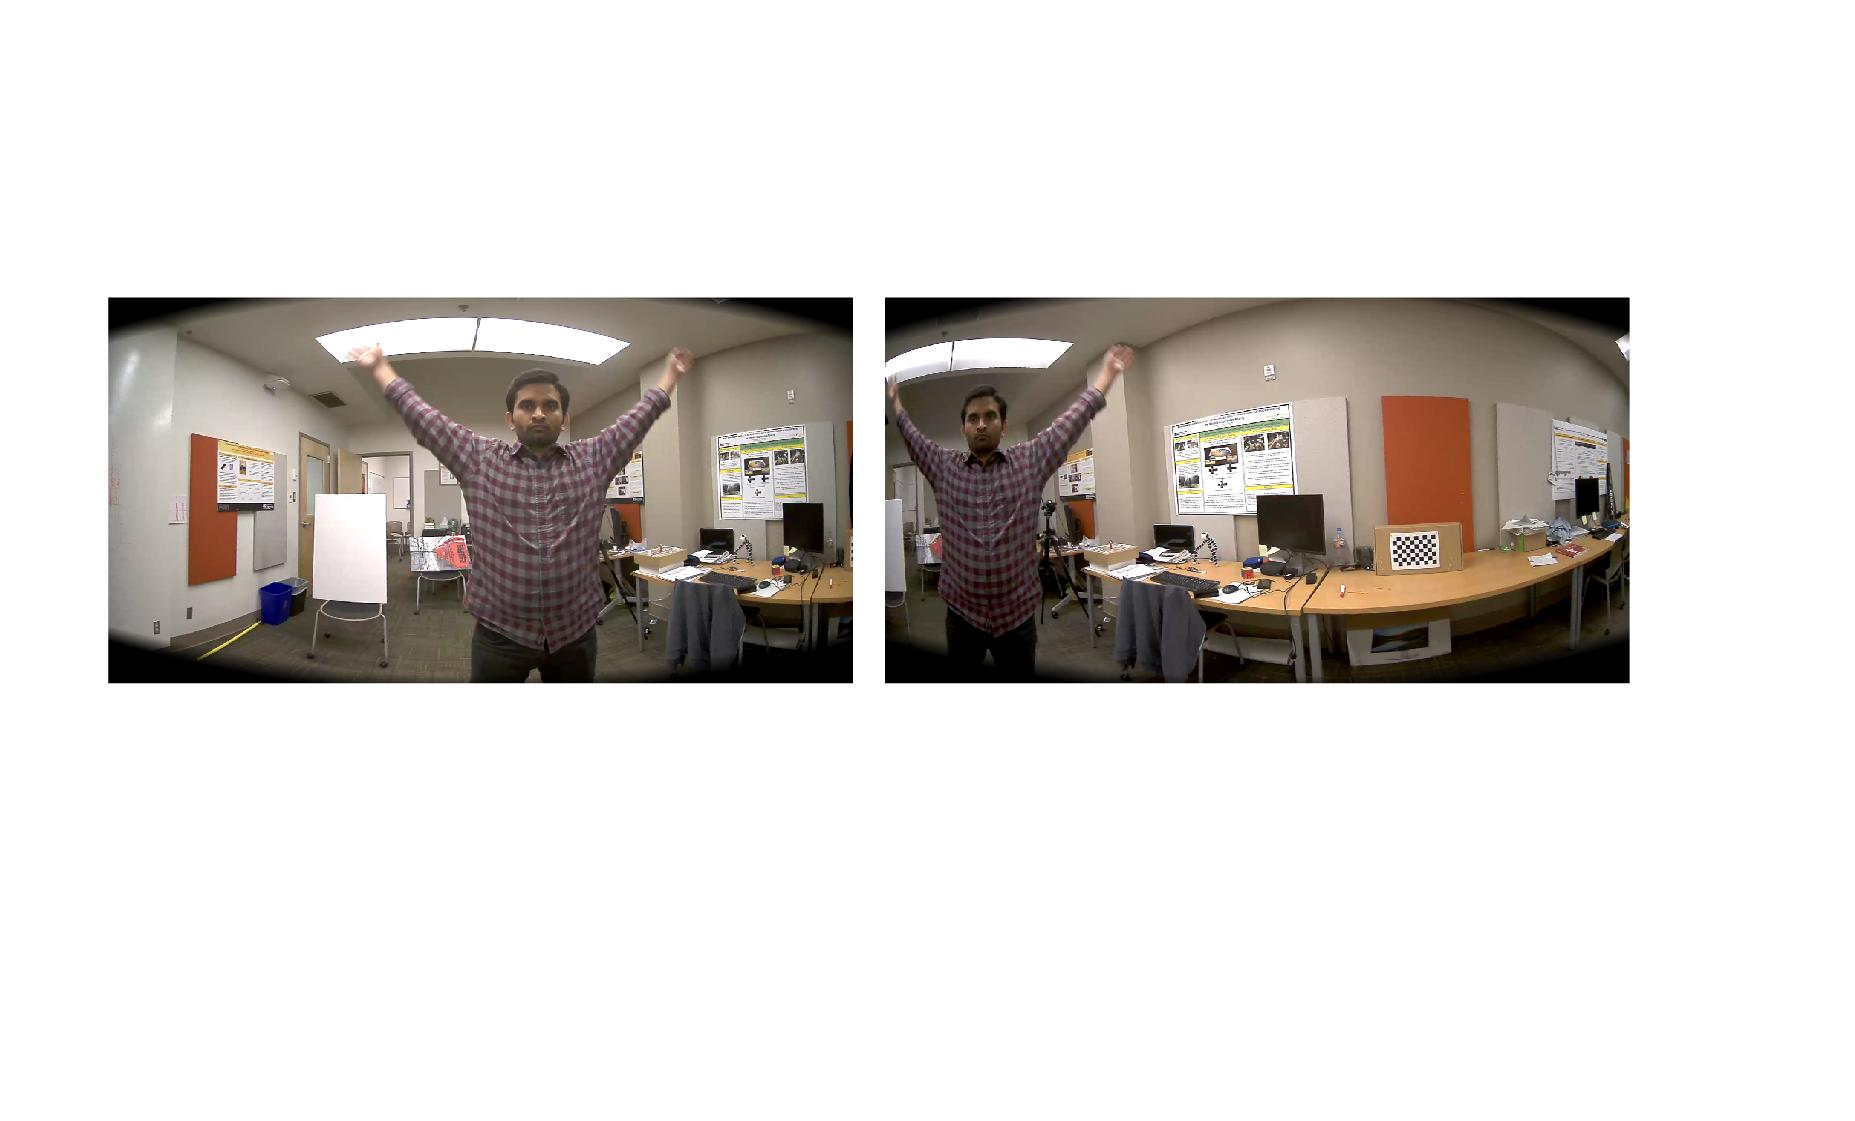
\includegraphics[width=1.1\textwidth]{/media/gunman/Data/thesis/ThesisLatex/data/images/EqRect_2_adj_images.jpg}
		\caption{Equirectangular Projection of first and second camera frames}
		\label{ODS_Input_Ouput}
	\end{center}
	\vspace{-0.3in}
\end{figure*} 

The overlapping left and right images.
\begin{figure*}
	\begin{center}
		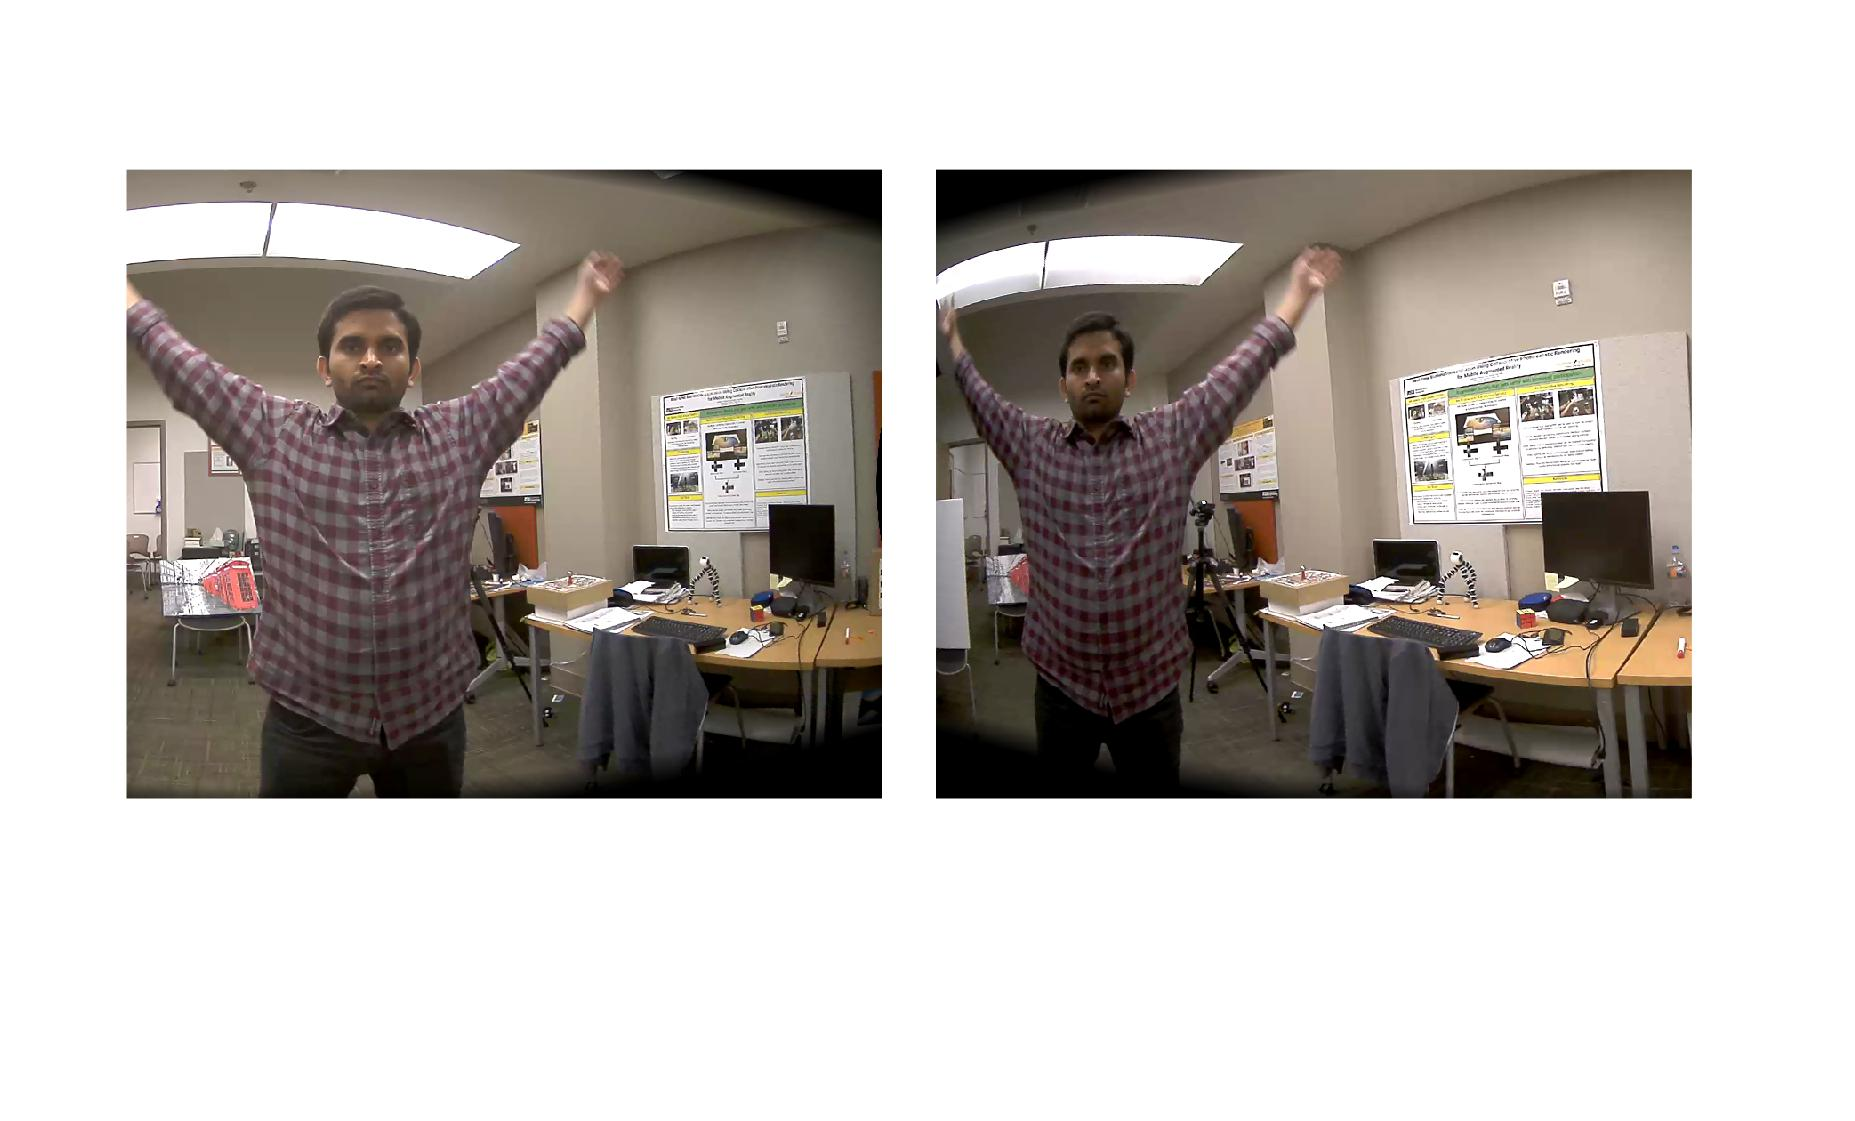
\includegraphics[width=1.1\textwidth]{/media/gunman/Data/thesis/ThesisLatex/data/images/OF_inp_overlap_region_of_adj_cam.jpg}
		\caption{Optical flow inputs: Overlapping regions of adjacent camera images. Equirectangular Projection of first and second camera frames}
		\label{ODS_Input_Ouput}
	\end{center}
	\vspace{-0.3in}
\end{figure*} 


\begin{figure*}
	\begin{center}
		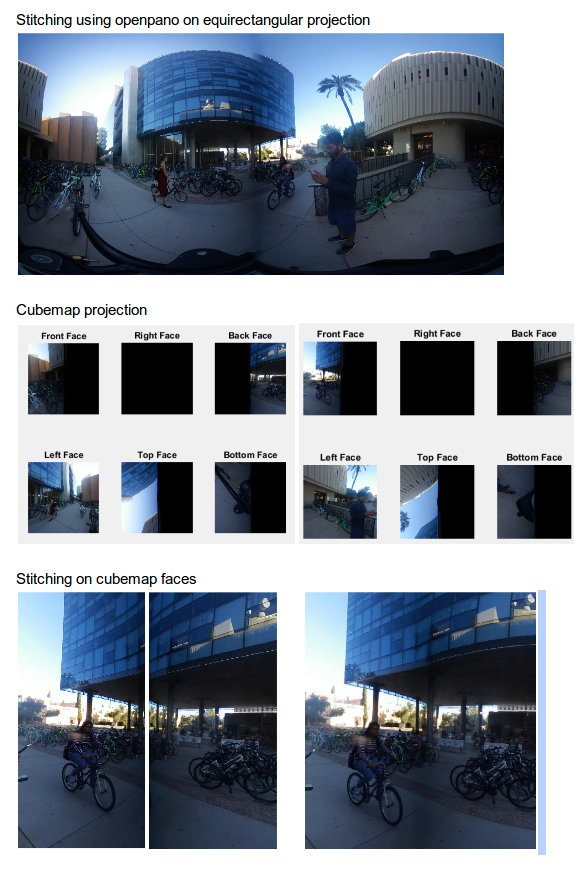
\includegraphics[width=1\textwidth]{/media/gunman/Data/thesis/ThesisLatex/data/images/CubeMapBasedStitching.png}
		\caption{Cubemap based Stitching, Path : /media/gunman/Data/fall-2017/research/mono360/equi2cubic}
		\label{ODS_Input_Output}
	\end{center}
	\vspace{-0.3in}
\end{figure*} 

Maximum Function For Extreme low power applications:
Since the alignment techniques is not the final algorithm I may be going ahead with, I want to start with something even simpler, i.e a maximum function. We can imagine the core computation block as a black box, that can be changes as per the needs of the application. This becomes an interesting use case as the final camera could have multiple such black boxes which can be turned on and off based on application demand. For eg. If the camera is being used for CNNs, maximum function might be good enough. If it’s going to be used for scene capture, then we can turn on an efficient stitching core instead of maximum function.





